\chapter{Introduction}

\section{Physics Motivation}

The existence of additional $U(1)$ gauge symmetries of nature are ubiquitous in
several Beyond the Standard Model (BSM) theories [].  

As Holdom \cite{holdom1986} realized in the mid eighties, in a theory with 
$U(1)_Y \times U(1)_D$, the gauge term of the Lagrangian can be written as 
\begin{equation}
    \mathcal{L}_{\text{gauge}} = - \frac{1}{4} F_Y^{\mu \nu}F_{Y, \mu \nu}
                          - \frac{1}{4} F'^{\mu \nu}F'_{\mu \nu}
                          + \frac{1}{2} \epsilon F'^{\mu \nu} F_{Y, \mu \nu}
    \label{eqn:l_gauge}
\end{equation}
%the associated gauge boson (heavy photon,
%dark photon or $A'$) can couple to the SM photon through the ``kinetic mixing''
%interaction
where $F'_{\mu \nu} = \partial_{\mu}A'_{\nu} - \partial_{\nu}A'_{\mu}$ 
($F^{\mu \nu}_{Y} = \partial^{\mu}A^{\nu} - \partial^{\nu}A^{\mu}$) is the
field strength tensor of the heavy photon (SM hypercharge) and $\epsilon$ is a
dimensionless coupling constant.  Decoupling of the fields can be achieved by 
shifting the SM hypercharge gauge field as 
\begin{equation}
    A_{\mu} \rightarrow A_{\mu} - \epsilon A'_{\mu}.
\end{equation}
This results in the diagnolization of \ref{eqn:l_gauge} as
\begin{equation}
    \mathcal{L}_{\text{gauge}} = - \frac{1}{4} F_Y^{\mu \nu}F_{Y, \mu \nu}
                          - \frac{1}{4} F'^{\mu \nu}F'_{\mu \nu}.
\end{equation}
However, the redefinition of the field also affects the interaction term of 
the Lagrangian
\begin{equation}
    \mathcal{L}_{int} 
\end{equation}
This, in turn, induces an effective coupling between the electromagnetic current
and the heavy photon field as 
\begin{equation}
    \mathcal{L}_{int} = \epsilon A'^{\mu}J_{\mu}^{EM}
\end{equation}
As explained below, this interaction can be exploited to search for heavy 
photons.

Several theories have envisioned scenarios generating 
$\epsilon \sim 10^{-6} - 10^{-2}$.

\section{Motivations for a Heavy Photon from Dark Matter}

Although the existence of dark matter (DM) has been firmly established through its
gravitational interaction \cite{popolo2014}, its exact nature continues to elude
us.  An appealing
possibility is that DM inhabits a ``hidden sector'' and interacts via a heavy
photon.  Their possible coupling can provide a portal that would allow the
exploration not only of the properties of DM but hidden sector itself.  Furthermore, such a
model may provide an explanation to several recently observed astrophysical
anomalies.  In fact, such anomalies have led to the conception of several DM
models involving the heavy photon.  A summary of those anomalies along with 
with their dark matter interpretation will be presented here.

\subsection{Cosmic Rays}

Interest in hidden sector models surged in 2008 with the announcement by 
The Payload for Antimatter Matter Exploration and Light-nuclei Astrophysics 
(PAMELA) of an unforeseen rise in the ratio of the cosmic ray (CR) positron flux
to CR electrons, $e^{+}/(e^{+} + e^{-})$, flux above 10 GeV \cite{pamela2008}.
The rise was later confirmed by both the 
Fermi Gamma-Ray Space Telescope \cite{Ackermann2012} and Alpha Magnetic 
Spectrometer-02 \cite{Aguilar2013} experiments and observed to continue
up to 200 GeV. The main source of CR positrons 
was expected to come from the interaction of CR nuclei with the interstellar 
medium (secondary production).  If such a production mechanism was dominant, 
cosmic ray propagation models predicted the fraction would fall with increasing
energy.  The observed rise lead to the speculation of additional sources of 
positrons including pulsars [?], supernova [?] and DM annihilation [?].

One attractive scenario that could account for the rise was the annihilation of
DM.  Specifically, models where DM annihilates to leptons ($e^+e^-, \mu^+\mu^-$)
where found to fit the data fairly well, although, they
require very large annihilaion rates \cite{Cholis2009}. Alternatively, a model
which envisions DM annihlating to a heavy photon which subsequently decays to 
$e^+e^-$ naturally leads to an enhacement in the 
annihilation cross-section \cite{Arkani-Hamed2009}.

\section{Current Limits on Heavy Photons}

\subsection{Electorn Beam Dump Experiments}

Electron beam dump experiments make use of a high intensity beam ``dumped'' onto
a ($\sim$ cm) target to produce highly boosted heavy photons through a process
analogous to photon bremstrahlung (see chapter 2).  In order to suppress the 
large SM background produced at the target, a shield ($\sim cm - m$) is usually
placed immediately downstream of the target and in front of the detector.  The
thickness of the target and shield along with the high luminosity allow such 
experiments to be sensitive to heavy photons with small couplings which tend to
travel considerable distances before decaying.  

Several beam dump experiments took place over the last decade. These include 
%E137 \cite{PhysRevD.38.3375} and E141 \cite{PhysRevLett.59.755} conducted at 
SLAC, 

\subsection{Electron Fixed Target Experiments}

\subsection{Proton Beam Dump Experiments}

\subsection{Electron-Positron Colliders}

\begin{figure}[t]
    \centering
    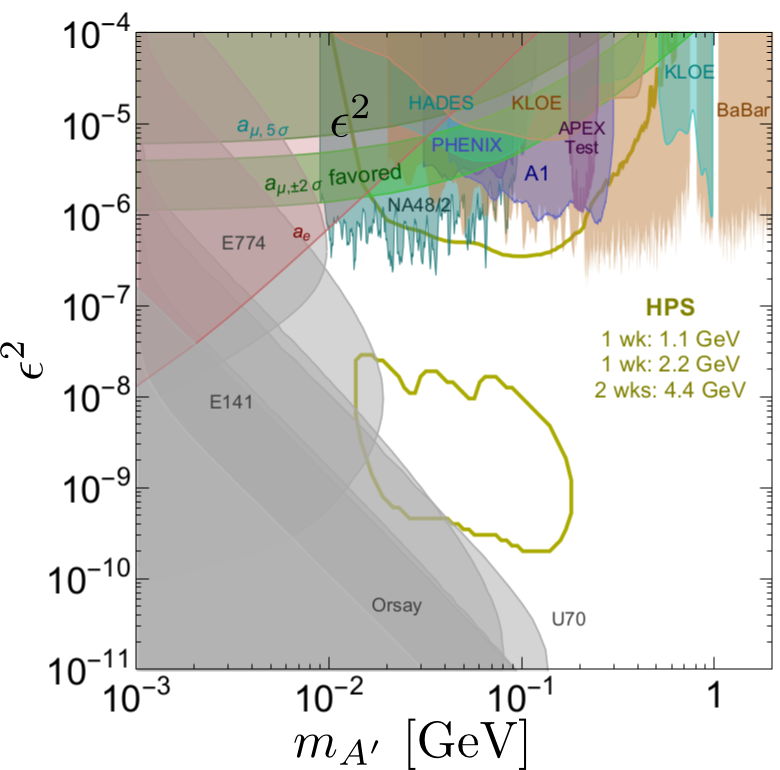
\includegraphics[width=0.9\textwidth]{images/ap_current_limits.png}
    \caption{Current limits on heavy photons.}
    \label{fig:svt_layout_render}
\end{figure}
